\documentclass{article}

\usepackage[english]{babel}
\usepackage[utf8]{inputenc}
\usepackage{amsmath,amssymb}
\usepackage{parskip}
\usepackage{graphicx}
\usepackage{listings}
\usepackage{float}
\usepackage{subfig}

\lstset{
    numbers=left, 
    numberstyle= \tiny, 
    keywordstyle= \color{ blue!70},
    commentstyle= \color{red!50!green!50!blue!50}, 
    frame=shadowbox, % 阴影效果
    rulesepcolor= \color{ red!20!green!20!blue!20} ,
    escapeinside=``, % 英文分号中可写入中文
    xleftmargin=2em,xrightmargin=2em, aboveskip=1em,
    framexleftmargin=2em,
    language = python,
    breaklines = true
} 
% Margins
\usepackage[top=2.5cm, left=3cm, right=3cm, bottom=4.0cm]{geometry}
% Colour table cells
\usepackage[table]{xcolor}

% Get larger line spacing in table
\newcommand{\tablespace}{\\[1.25mm]}
\newcommand\Tstrut{\rule{0pt}{2.6ex}}         % = `top' strut
\newcommand\tstrut{\rule{0pt}{2.0ex}}         % = `top' strut
\newcommand\Bstrut{\rule[-0.9ex]{0pt}{0pt}}   % = `bottom' strut

%%%%%%%%%%%%%%%%%
%     Title     %
%%%%%%%%%%%%%%%%%
\title{CSCI803 Assignment}
\author{Yao Xiao \\ SID 2019180015}
\date{\today}

\begin{document}
\maketitle

%%%%%%%%%%%%%%%%%
%   Problem 1   %
%%%%%%%%%%%%%%%%%
\section{Problem Description}
In fact, we are inseparable from the web page every day. How to efficiently and accurately give the ranking of the web page or give the relevant page list is what I want to discuss and solve.

\section{Solution}
\subsection{Strategy 1} 
First of all, give the core idea.

\begin{enumerate}
    \item If a page is linked by many other pages, it means that the page is more important, that is, the PageRank value will be relatively high.
    \item If a page with a high PageRank value links to another page, the PageRank value of the linked page will increase accordingly.
\end{enumerate}

The Internet can be regarded as a directed graph, each web page is a node of the digraph, and each hyperlink between the web pages is an edge of the digraph.

\begin{figure}[H]
    \centering
    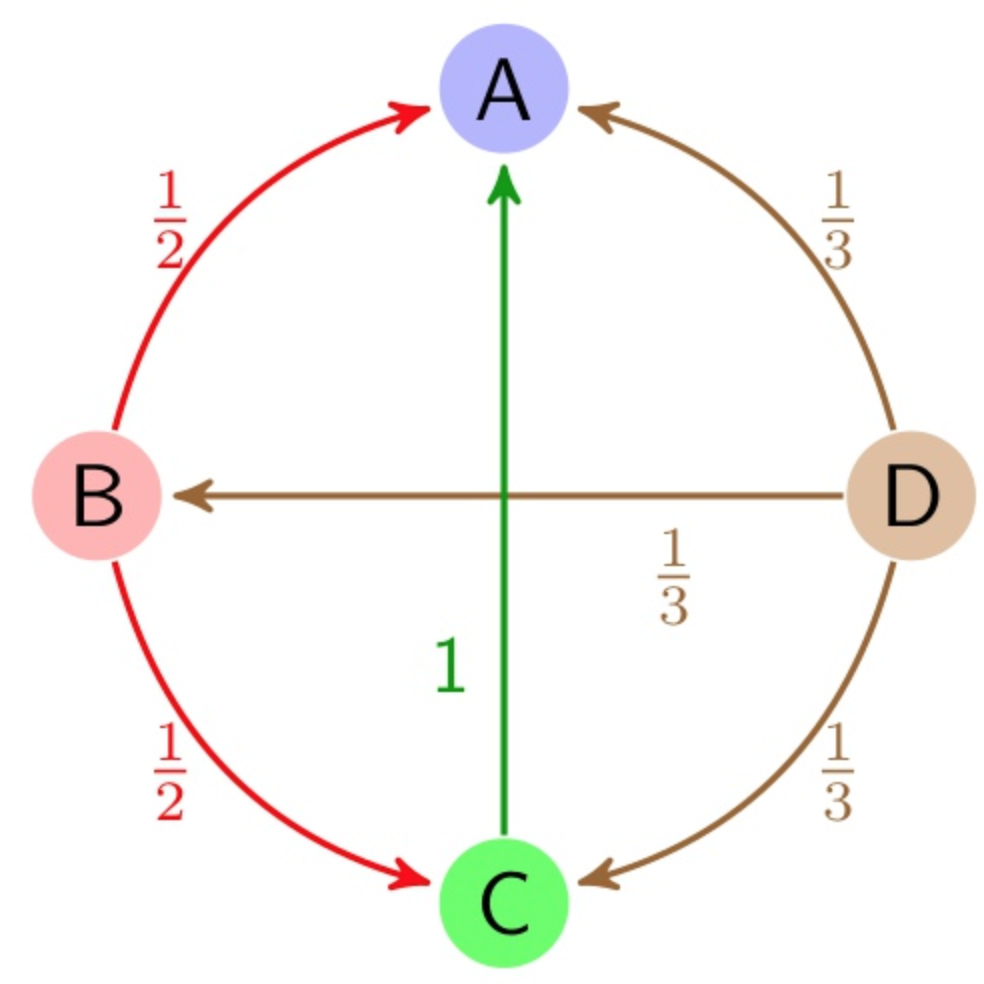
\includegraphics[width=0.4\textwidth]{Fig1}
\end{figure}

The R value of a will be the sum of the R values of B, C and D pages, but other nodes still have links to different nodes. So we can get the formula:
\begin{equation}
    \begin{aligned}
        R(A) &= \frac{R(B)}{2} + \frac{R(C)}{2} + \frac{R(D)}{3}\\
        R(u) &= \sum_{v\in B_{u}} \frac{R(v)}{L(v)}
    \end{aligned}
\end{equation}

$B_u$ is a collection of all web pages linked to web page $u$, 
web page $v$ is a web page belonging to the collection $B_u$,
and $L(v)$ is the number of external links to the web page $v$ (that is, out-degree).

In the Internet, a web page only has its own chain, or a few pages out of the chain to form a circle. Then, in the process of continuous iteration, the R value of one or several pages will only increase but not decrease.
So we can further define it as:
\begin{equation}
    R(p_i) = \frac{1-d}{N} + d \sum_{p_j\in M(p_i)} \frac{R(p_j)}{L_n(p_j)}
\end{equation}

$d$ is called damping factor, which means the probability that a user reaches a page and continues to browse backward at any time.
The matrix form of the above formula is:

\begin{figure}[H]
    \centering
    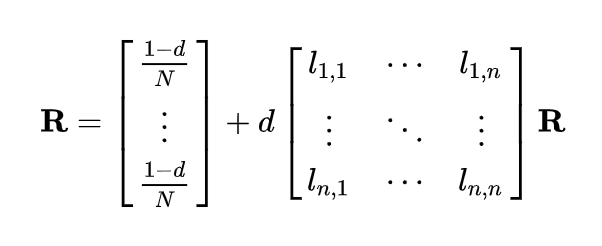
\includegraphics[width=0.4\textwidth]{Fig2}
\end{figure}

Then through $R_{n+1} = AR_{n}$ iterate continuously the PR value,
when the following inequality is satisfied, the iteration ends and the PR values of all pages are obtained:
\begin{equation}
    |R_{n+1} - R_n | < \epsilon 
\end{equation}

In summary, a random walk model is defined on a directed graph, that is, a first-order Markov chain, which describes the behavior of random walkers randomly visiting each node along the directed graph. Under certain conditions, the probability of visiting each node in the extreme case converges to a stable distribution. At this time, the stable probability value of each node is its PageRank value, which indicates the importance of the node.

\subsection{Strategy 2}
At the very beginning, we need to understand two properties. "Authority webpage": For a specific search, this webpage provides the best relevant information; "Hub webpage": This webpage provides many hyperlinks to other authoritative webpages.

The core idea is:
\begin{enumerate}
    \item A good Hub web page points to a good Authority web page.
    \item A good Authority webpage is directed by a good Hub-type webpage.
\end{enumerate}

First, the query q is submitted to the retrieval system based on keyword query, and the first n web pages are always taken from the set of returned result pages, as the root set, denoted as $S$.
By adding web pages referenced by S and web pages referencing to S, expand S into a larger set T. Take the Hub web page in T as the node set $V1$ and the authoritative web page as the node set $V2$.
The hyperlink from the web page in $V1$ to the web page in $V2$ is the edge set E, forming a bipartite directed graph. For any node $v$ in $V1$, use $h(v)$ to denote the Hub value of web page $v$, and $h (v)$ Convergence; for the vertex $u$ in $V2$, use $a (u)$ to represent the authority value of the web page.
At the beginning, $h(u) = a(u) = 1$, and then we start the iterative process:
\begin{equation}
    \forall u, a(u) = \sum^n_{i=1} h(u)
\end{equation}

\begin{equation}
    \forall u, h(u) = \sum^n_{i=1} a(u)
\end{equation}

At the end of each iteration, standardization is required:
\begin{equation}
    \sum^n_{i=1}h(i)^2 = \sum^n_{i=1}a(i)^2 = 1
\end{equation}

We can set an upper limit of the number of iterations k to control, or set a threshold, when the change is less than the threshold, the iteration ends. Then just return to the top dozen or so pages of the user’s authority value.

From the perspective of the two types of weight propagation, the first strategy is based on the random walk model, which directly transmits the weight of the webpage from the authority webpage to the authority webpage; and the second strategy is to spread the weight of the authority webpage through the hub webpage.

From the point of view of algorithm, although both are link analysis algorithms, there are still some differences between the two. The principle of strategy two is as mentioned above, its authority value is only relative to the weight of a certain retrieval subject, while strategy one is independent retrieval subject.

\section{Experimental Results}
\subsection{Strategy 1}
\begin{lstlisting}
from pygraph.classes.digraph import digraph

class PRIterator:
    __doc__ = "calculate the PR of a graph"
    def __init__(self, dg):
        self.damping_factor = 0.85 
        self.max_iterations = 100  
        self.min_delta = 0.00001
        self.graph = dg

    def page_rank(self):
        for node in self.graph.nodes():
            if len(self.graph.neighbors(node)) == 0:
                for node2 in self.graph.nodes():
                    digraph.add_edge(self.graph, (node, node2))

        nodes = self.graph.nodes()
        graph_size = len(nodes)

        if graph_size == 0:
            return {}
        page_rank = dict.fromkeys(nodes, 1.0 / graph_size)  
        # (1 - \alpha) / N
        damping_value = (1.0 - self.damping_factor) / graph_size  

        flag = False
        for i in range(self.max_iterations):
            change = 0
            for node in nodes:
                rank = 0
                for incident_page in self.graph.incidents(node): 
                    rank += self.damping_factor * (page_rank[incident_page] / len(self.graph.neighbors(incident_page)))
                rank += damping_value
                change += abs(page_rank[node] - rank) 
                page_rank[node] = rank

            print("This is NO.%s iteration" % (i + 1))
            print(page_rank)

            if change < self.min_delta:
                flag = True
                break
        if flag:
            print("finished in %s iterations!" % node)
        else:
            print("finished out of 100 iterations!")
        return page_rank


if __name__ == '__main__':
    dg = digraph()

    dg.add_nodes(["A", "B", "C", "D", "E"])

    dg.add_edge(("A", "B"))
    dg.add_edge(("A", "C"))
    dg.add_edge(("A", "D"))
    dg.add_edge(("B", "D"))
    dg.add_edge(("C", "E"))
    dg.add_edge(("D", "E"))
    dg.add_edge(("B", "E"))
    dg.add_edge(("E", "A"))

    pr = PRIterator(dg)
    page_ranks = pr.page_rank()

    print("The final page rank is\n", page_ranks)

\end{lstlisting}

\begin{figure}[H]
    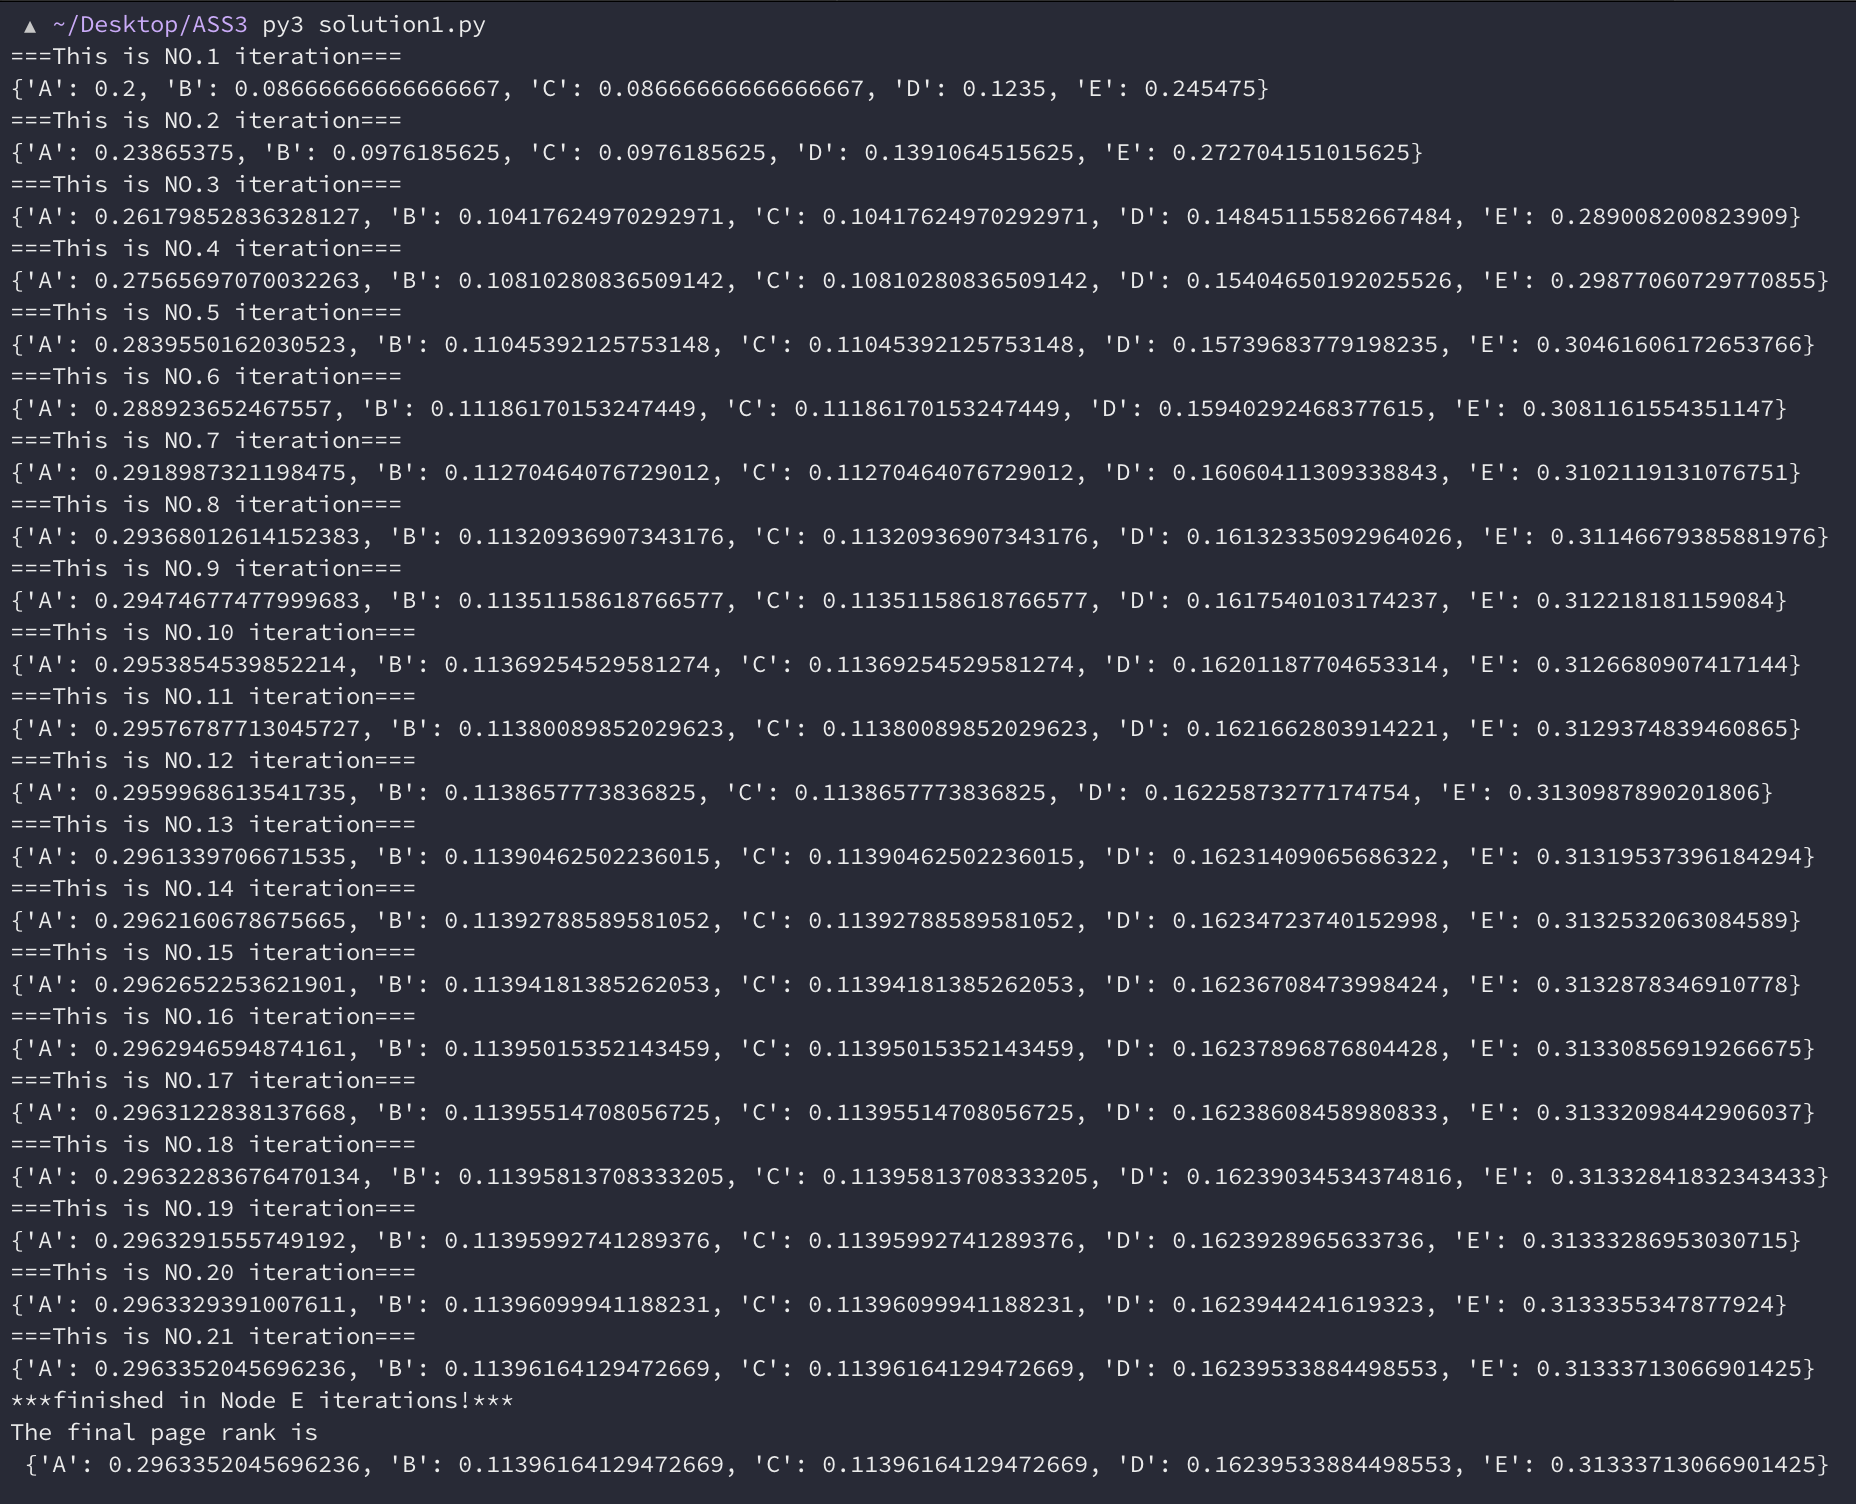
\includegraphics[width=1\textwidth]{Fig3}
\end{figure}

\subsection{Strategy 2}
\begin{lstlisting}
from pygraph.classes.digraph import digraph
from math import sqrt

class HITSIterator:
    __doc__ = "calculate the Hup and Authority value of a graph"

    def __init__(self, bg):
        self.max_iterations = 100  
        self.min_delta = 0.0001  
        self.graph = bg

        self.hub = {}
        self.authority = {}
        for node in self.graph.nodes():
            self.hub[node] = 1
            self.authority[node] = 1

    def hits(self):
        if not self.graph:
            return

        flag = False
        for i in range(self.max_iterations):
            change = 0.0 
            norm = 0  
            tmp = {}
            tmp = self.authority.copy()
            for node in self.graph.nodes():
                self.authority[node] = 0
                for incident_page in self.graph.incidents(node):  
                    self.authority[node] += self.hub[incident_page]
                norm += pow(self.authority[node], 2)
            norm = sqrt(norm)
            for node in self.graph.nodes():
                self.authority[node] /= norm
                change += abs(tmp[node] - self.authority[node])

            # calculate the hup value of each page
            norm = 0
            tmp = self.hub.copy()
            for node in self.graph.nodes():
                self.hub[node] = 0
                for neighbor_page in self.graph.neighbors(node):  
                    self.hub[node] += self.authority[neighbor_page]
                norm += pow(self.hub[node], 2)
            # normalization 
            norm = sqrt(norm)
            for node in self.graph.nodes():
                self.hub[node] /= norm
                change += abs(tmp[node] - self.hub[node])

            print("====This is NO.%s iteration===" % (i + 1))
            print("@authority", self.authority)
            print("@hub", self.hub)

            if change < self.min_delta:
                flag = True
                break
        if flag:
            print("***finished in %s iterations!***" % (i + 1))
        else:
            print("***finished out of 100 iterations!***")

        print("The best authority page: ", max(self.authority.items(), key=lambda x: x[1]))
        print("The best hub page: ", max(self.hub.items(), key=lambda x: x[1]))


if __name__ == '__main__':
    bg = digraph()

    bg.add_nodes(["A", "B", "C", "D", "E"])

    bg.add_edge(("A", "C"))
    bg.add_edge(("A", "D"))
    bg.add_edge(("B", "D"))
    bg.add_edge(("C", "E"))
    bg.add_edge(("D", "E"))
    bg.add_edge(("B", "E"))
    bg.add_edge(("E", "A"))

    hits = HITSIterator(bg)
    hits.hits()
\end{lstlisting}

\begin{figure}[H]
    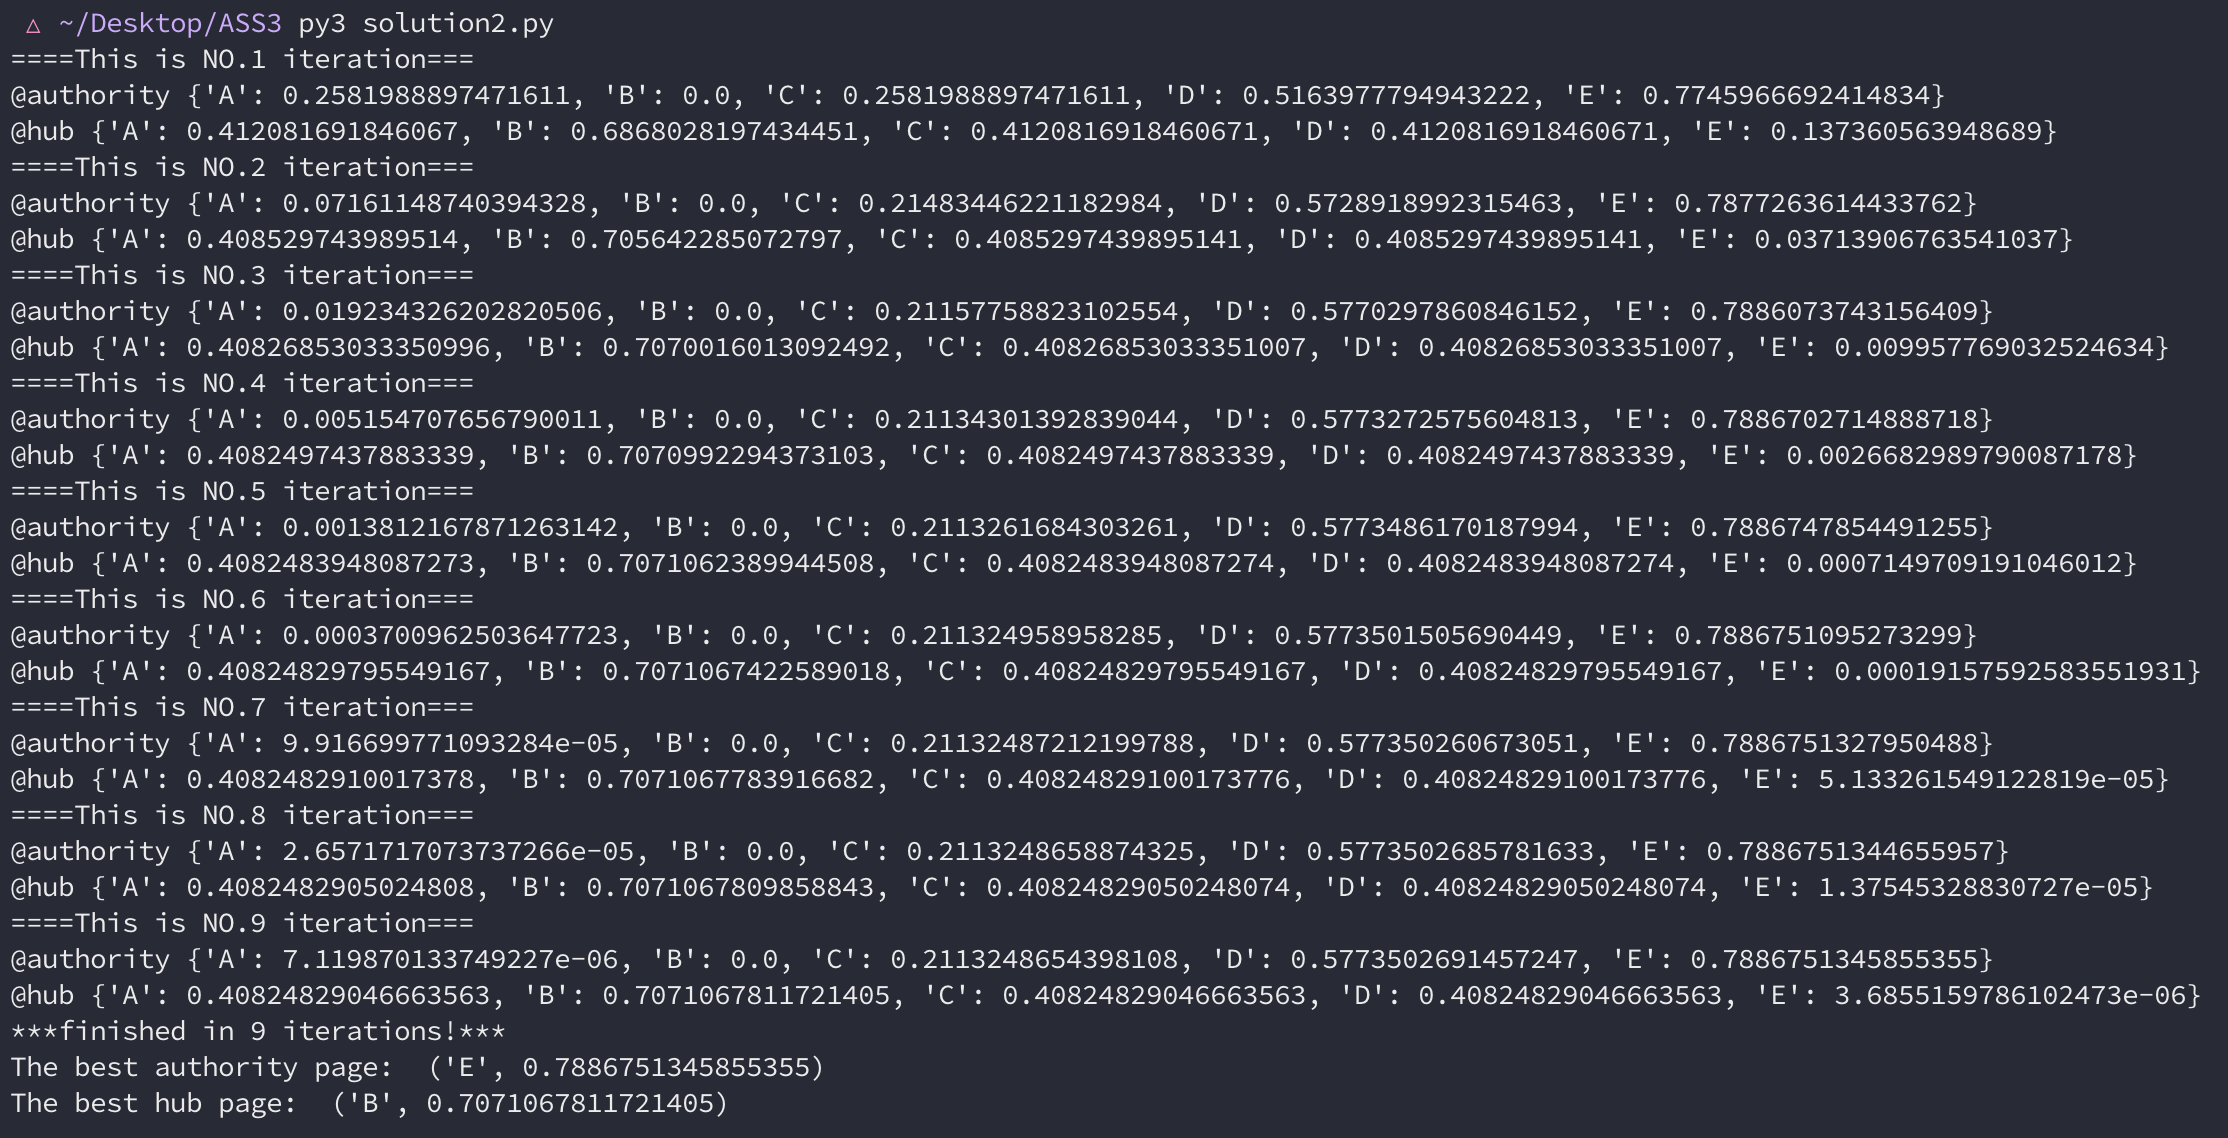
\includegraphics[width=1\textwidth]{Fig4}
\end{figure}
\end{document}
